\let\negmedspace\undefined
\let\negthickspace\undefined
\documentclass[journal,12pt,onecolumn]{IEEEtran}
\usepackage{cite}
\usepackage{amsmath,amssymb,amsfonts,amsthm}
\usepackage{algorithmic}
\usepackage{graphicx}
\usepackage{textcomp}
\usepackage{xcolor}
\usepackage{txfonts}
\usepackage{listings}
\usepackage{enumitem}
\usepackage{mathtools}
\usepackage{gensymb}
\usepackage{comment}
\usepackage[breaklinks=true]{hyperref}
\usepackage{tkz-euclide} 
\usepackage{listings}
\usepackage{gvv}                                        
%\def\inputGnumericTable{}                                 
\usepackage[latin1]{inputenc}                                
\usepackage{color}                                            
\usepackage{array}                                            
\usepackage{longtable}                                       
\usepackage{calc}                                             
\usepackage{multirow}                                         
\usepackage{hhline}                                           
\usepackage{ifthen}                                           
\usepackage{lscape}
\usepackage{tabularx}
\usepackage{array}
\usepackage{float}


\newtheorem{theorem}{Theorem}[section]
\newtheorem{problem}{Problem}
\newtheorem{proposition}{Proposition}[section]
\newtheorem{lemma}{Lemma}[section]
\newtheorem{corollary}[theorem]{Corollary}
\newtheorem{example}{Example}[section]
\newtheorem{definition}[problem]{Definition}
\newcommand{\BEQA}{\begin{eqnarray}}
\newcommand{\EEQA}{\end{eqnarray}}
\newcommand{\define}{\stackrel{\triangle}{=}}
\theoremstyle{remark}
\newtheorem{rem}{Remark}
\begin{document}
\bibliographystyle{IEEEtran}
\vspace{3cm}

\title{1.5.19}
\author{EE24BTECH11003 - Akshara Sarma Chennubhatla}
\maketitle
\bigskip

\renewcommand{\thefigure}{\theenumi}
\renewcommand{\thetable}{\theenumi}

\textbf{Question:} \\Find the ratio in which the segment joining the points \brak{1,3} and \brak{4, 5} is divided by the $X$ axis. Also find the coordinates of this point on the $X$ axis.
Using section formula,\\
\solution
\begin{align}
\myvec{x\\0}&=\frac{\myvec{1\\3}+k\myvec{4\\5}}{1+k}\\
\implies \frac{5k+3}{k+1}&=0\\
\implies k&=\frac{-3}{5}\\
x&=\frac{1}{k+1}+\frac{4k}{k+1}\\
\implies x&=\frac{1+4\brak{\frac{-3}{5}}}{\brak{\frac{-3}{5}}+1}\\
\implies x&=\frac{-7}{2}
\end{align}
Therefore the ratio in which the line segment joining the points \brak{1,3} and \brak{4,5} is divided by the $X$ axis is $-3:5$. The point on the $X$ axis which divides the line segment in the ratio is $\brak{\frac{-7}{2},0}$
\begin{figure}[h!]
\centering
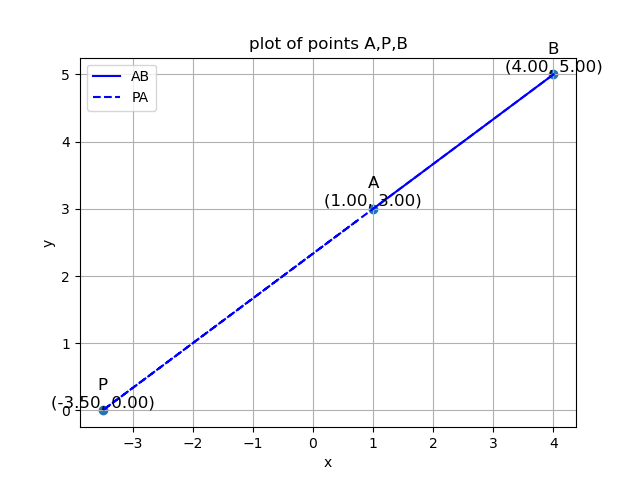
\includegraphics[width=0.7\linewidth]{figs/figure.png}	
\label{stemplot}
\end{figure}
\end{document}

